% !TEX TS-program = xelatex
\documentclass[12pt,a4paper]{article}

% Packages
\usepackage{geometry}
\usepackage{fontspec}
\usepackage{tikz}
\usepackage{fancyhdr}
\usepackage{setspace}
\usepackage{titlesec}
\usepackage{eso-pic}


% Page geometry
\geometry{
  top=2cm,
  bottom=2cm,
  left=3cm,
  right=3cm
}


% Fonts
\setmainfont{Georgia}
\newfontfamily\futurafont{Futura}

% Line spacing
\onehalfspacing

% Header and footer setup
\pagestyle{fancy}
\fancyhf{}
\fancyheadoffset[L]{+1.5cm}
\fancyheadoffset[R]{+1.5cm}
\fancyfootoffset[L]{+1.5cm}
\fancyfootoffset[R]{+1.5cm}
% Header content (dynamic from YAML)
%\fancyhead[L]{\futurafont\small $}
\fancyhead[C]{\futurafont\small xtitle: coherence \& presuppositions observations in :schizophrenia: threads}
\fancyhead[R]{\futurafont\small st. schwarz}
%\fancyhead[R]{\futurafont\small }

% Footer content (dynamic)
\fancyfoot[R]{\futurafont\small  \hspace{1em} | \hspace{1em} 2025-10-11}

% Remove default header/footer lines
\renewcommand{\headrulewidth}{0pt}
\renewcommand{\footrulewidth}{0pt}

% Draw decorative boxes/lines from Quark layout
\AddToShipoutPictureBG*{%
  \begin{tikzpicture}[remember picture, overlay]
    % --- Header lines ---
   % \draw[line width=0.4pt]
    %  ([xshift=1cm,yshift=-1.5cm]current page.north west)
     % -- ([xshift=-1cm,yshift=-1.5cm]current page.north east);
    %\draw[line width=0.4pt]
     % ([xshift=1cm,yshift=-1.9cm]current page.north west)
      %-- ([xshift=-1cm,yshift=-1.9cm]current page.north east);

    % --- Footer lines ---
    %\draw[line width=0.4pt]
     % ([xshift=1cm,yshift=2cm]current page.south west)
      %-- ([xshift=-1cm,yshift=2cm]current page.south east);
   % \draw[line width=0.4pt]
    %  ([xshift=0.8cm,yshift=2.4cm]current page.south west)
     % -- ([xshift=-0.8cm,yshift=2.4cm]current page.south east);

    % --- Metadata box (upper left) ---
  %  \draw[line width=0.3pt]
   %   ([xshift=1cm,yshift=-3.5cm]current page.north west);
%      rectangle ([xshift=5cm,yshift=-6.5cm]current page.north west);

    % --- Corner decorations ---
    \draw[line width=1.3pt]
      ([xshift=0.7cm,yshift=-0.6cm]current page.north west)
      -- ++(0,-0.8cm) -- ++(20cm,0);
    \draw[line width=1.3pt]
      ([xshift=-0.7cm,yshift=-0.6cm]current page.north east)
      -- ++(0,-0.8cm) -- ++(-0.8cm,0);
    \draw[line width=1.3pt]
      ([xshift=0.7cm,yshift=0.8cm]current page.south west)
      -- ++(0,0.8cm) -- ++(0.8cm,0);
    \draw[line width=1.3pt]
      ([xshift=-0.7cm,yshift=0.8cm]current page.south east)
      -- ++(0,0.8cm) -- ++(-20cm,0);
  \end{tikzpicture}
}

% Title formatting
\titleformat{\section}{\normalfont\bfseries\large}{\thesection.}{1em}{}

% Document start
\begin{document}

% Optional dynamic header box content
%  {\futurafont\small  |  | 2025-10-11}
%\end{flushleft}

\vspace{1cm}

% Main content area
\chapter{index}\label{index}

linguistics, AVL, alii pub essais extension.

\begin{Shaded}
\begin{Highlighting}[]
\CommentTok{\#dataset\textless{}{-}7}
\CommentTok{\#prelim}
\end{Highlighting}
\end{Shaded}

\chapter{15303.ha.draft}\label{ha.draft}

\section{subject}\label{subject}

In this paper we want to explore \textbf{reference marking, coherence and information structure in schizophrenia language} by measuring distance of similar nouns preceded by specified determinants.\footnote{only according to the LLM training data, which is still a blackbox}\\
Inspired by Zimmerer et al. (\citeproc{ref-zimmerer_deictic_2017}{2017}) we are interested in observations concerning coherence and propositional statement conditions in schizophrenia language, as these linguistic markers appear underinvestigated in that fields research whilst they seem to play a crucial role within target group language features. (As such seen as asset of thinking or world building capacity which might suffer from linguistic standard deviation within the range of positive symptoms.) There seems to be a lot research done concerning frequency based analyses of how typical patients language might appear and how that language deviates in terms of keywords or word fields, but our interest is more directed onto the structural layer of the language which might not be catched by raw frequencies. In our opionion disturbances on that layer might even be hidden and not to grasp easily such that a listener would not always be able to precisely declare what the disturbing factor is. Missing \textbf{coherence}, which we will investigate, may be a too narrow explanation to many impressions that schizophrene language leaves the listener with. But it seems to be a good starting point to unveiling structural patterns of patients language.

\section{definitions, terminology, assumptions}\label{definitions-terminology-assumptions}

\subsection{coherence}\label{coherence}

There are several preliminary affordances to a successful communication. One is the \emph{coherence} of a \href{}{text = way of communication}, which accounts for the partner being able to follow the topic and relate subjects and objects referenced. There can be more or less \emph{common} references and such, that need to be embedded in context to be understood. The underlying network of informations to create that context is what we call \emph{information structure} of a text. The level of complexity of that network defines how simple it would be to gather the reference from the given information. We might have to go back many sentences or even infer reference from metaphors or such to be able to understand what is said while in the other case simply recall the subject of the last sentence to get the meaning (reference) of the pronoun in \texttt{also\ \{she\}\ said\ thisandthat...}.
The capacity to imagine or have in mind, what concrete information is accessible to the adressee (what he actually knows or can infer) is key to a successful communication, since factors like common-ness, weltwissen and shared knowledge between adressant and adressee and informations accessible from the text itself vary depending on topic, setting, intimacy of the partners and such. So one cannot always be sure that the information provided is sufficient but the grade to which one can give a correct estimate to this sufficiency should here be a measure for our hypothesis, that the very coherence in disturbed language is deficient which lets an utterance be more difficult to understand within the frame of given information.
Now one indicator of coherence we assume is \emph{reference distance} where according to our hypothesis a larger distance would be observed in places where the adressant overestimates\footnote{where ``obs'' comes first} the ability of the partner to follow a reference. That would mean that we find a medium shorter distance between referent and reference in the reference corpus\footnote{where the participants may show a more realistic estimation of beforementioned ability} and larger distances in the target corpus. The references we are interested in are nouns that appear as anaphors i.e.~here as noun analogies. The assumption is that if a noun is repeated \emph{and} is combinded with certain preceding determiners, the speaker assumes that the adressee has some knowledge of what is talked about, depending on the strength of the determination. So e.g.~\href{}{this, that, those, these} would be rather strong determiners requiring that the noun was introduced before; these are four determiners of our 5 conditions as listed below.

\subsection{premises}\label{premises}

\subsubsection{deictic anchoring and propositional complexity}\label{deictic-anchoring-and-propositional-complexity}

Zimmerer et al. (\citeproc{ref-zimmerer_deictic_2017}{2017}) consider
``Deictic anchoring {[}\ldots{]} an inherent part of the process by which we make references to aspects in the world including entities, events, locations, and time.'' and define propositions as being ``statements about the world which can be true or false.'' They mention, according to (\citeproc{ref-kuperberg_language_2010}{Kuperberg 2010}) ``that in people with schizophrenia, cortical activity to semantic abnormalities in sentences is particularly small compared to controls if interpretation requires integration of several sentences'' which can mean, that patients are not realising if their utterances are somehow disturbed on the semantics level.
If ``Delusions and thought disorder can be considered disruptions of propositional meaning'' then the patients feeling for their stated propositions (required to the adressee) and further the estimation about what he/she can assume as familiar to the adressee can be wrong. Following Klaus Konrad (\citeproc{ref-mishara_klaus_2010}{Mishara 2010}) who ``described the onset of a delusion as the loss of ability to transcend an experience and see it with the eyes of others'' Zimmerer et al. (\citeproc{ref-zimmerer_deictic_2017}{2017}) assume that ``in thought disorder, the ability to express coherent propositions can be severely impaired.'' We take that as premise for our research question.

\section{questions}\label{questions}

Measuring the referent-reference distance which we assume as an indicator for coherence we hope to find empirical evidence for disturbed or not world building capacities within schizophrenia language. Premising that a large noun distance indicates a low reference-referent association we hypothesise that in a language/ToM setting where the speakers estimation of the audiences context understanding capacities is disturbed we will find higer medium scores for the distance under matching conditions. An environment which has potential to test our hypothesis is the reddit thread r/schizophrenia. As reference corpus we chose reddit r/unpopularopinion.
The distance measured should give us information structural evidence of how strong the noun occurences\footnote{preceded by conditioned determiners} are connected, i.e.~if a noun appears out of the blue mostly or if it somewhere before has been introduced to the audience and thus would be more or less legitimated to be determined by an antecedent.
Our basic assumptions rely on the \emph{taxonomy of given end new information} coined by Prince (\citeproc{ref-prince_toward_1981}{1981}). She develops a hierarchy of references(fn:informations in a text) with specific relations to each other, where each item is attributed in terms of \emph{familiarity}\footnote{cf.~Prince: speaker assumptions about hearer familiarity = assumed familiarity}, that defines ranges of 1. givennes in the sense of predictability/recoverability, 2. givenness in the sense of saliency, 3. givenness in the sense of ``shared knowledge''. (cf. Prince (\citeproc{ref-prince_toward_1981}{1981}), pp.~226) We base our hypothesis of \emph{reference distance as indicator for coherence} on this model assuming that the reference/association strength\footnote{which should be weaker with growing distance between reference-referent} determines the level of text coherence.

\section{data}\label{data}

We built a corpus of the reddit r/schizophrenia thread (\texttt{n=1500371\ tokens}) and a reference corpus of r/unpopularopinion (\texttt{n=980731\ tokens}). Both were pos-tagged using the R udpipe package (Wijffels (\citeproc{ref-wijffels_udpipe_2023}{2023})) which tags according to the universal dependencies tagset maintained by De Marneffe et al. (\citeproc{ref-de_marneffe_universal_2021}{2021}). Still the available data can only, within the pipeline of steadily growing the corpus and devising the noun distances developed be just a starting point from where with more datapoints statistical evaluation becomes relevant.\\
The dataframe used for our model (actual: M13) consists of \texttt{142321} distance datapoints (sample Tab.X below) derived from the postagged corpus. Because the ranges of the url threads vary heavily between target and reference corpus, the distances are (in M13) normalised to the target corpus (cf.~Tab.X for the raw vs.~normalised distances comparison.) Outliers are excluded from the analysis since they very probably do not fulfill to can be counted as anaphoric references.

\resizebox{\ifdim\width>\linewidth\linewidth\else\width\fi}{!}{
\begin{tabular}{lllrlrrlrrrrrrrrr}
\toprule
token & upos & target & pos & prepos & url\_id & range & q & det & aut\_id & total\_mentions & dist & embed.score & dist\_rel\_within & dist\_rel\_all & dist\_rel\_obs & dist\_rel\_ref\\
\midrule
people & NOUN & obs & 270314 & ADV & 472 & 2845 & a & 0 & 153 & 10 & 122 & 0.380 & 82 & 137 & 82 & 192\\
things & NOUN & obs & 695454 & ADP & 1033 & 587 & a & 0 & 402 & 3 & 94 & 0.337 & 305 & 513 & 305 & 718\\
languages & NOUN & ref & 377661 & ADV & 2009 & 1735 & a & 0 & 5539 & 13 & 199 & 0.271 & 514 & 368 & 218 & 514\\
meds & NOUN & obs & 782641 & ADP & 1218 & 1028 & a & 0 & 584 & 2 & 440 & 0.570 & 814 & 1372 & 814 & 1920\\
symptoms & NOUN & obs & 250787 & NOUN & 454 & 5112 & a & 0 & 23 & 13 & 92 & 0.430 & 34 & 58 & 34 & 81\\
\addlinespace
types & NOUN & obs & 596842 & DET & 873 & 3756 & b & 1 & 127 & 4 & 587 & 0.319 & 297 & 501 & 297 & 701\\
state & NOUN & ref & 642972 & VERB & 2133 & 5094 & a & 0 & 5811 & 6 & 83 & 0.371 & 73 & 52 & 31 & 73\\
hotline & NOUN & obs & 1075076 & NOUN & 1625 & 444 & a & 0 & 2198 & 3 & 12 & 0.585 & 51 & 87 & 51 & 121\\
time & NOUN & ref & 49023 & VERB & 1876 & 1798 & a & 0 & 3800 & 8 & 36 & 0.378 & 90 & 64 & 38 & 90\\
love & NOUN & obs & 861296 & ADP & 1338 & 3513 & a & 0 & 2119 & 18 & 2 & 0.459 & 1 & 2 & 1 & 3\\
\bottomrule
\end{tabular}}

\section{methods}\label{methods}

To compute distances we queried the corpus for matching conditions where certain (probable) determiners appear before analogue nouns (anaphors). For each datapoint we collect variables as:

\begin{itemize}
\tightlist
\item
  thread url
\item
  author (anonymised)
\item
  thread length (tokens)
\item
  lexical diversity (type/token ratio)
\item
  lemma
\item
  distance (to the preceding occurence, e.g.~for three occurences of \href{}{dog} we collect 2 distance datapoints)
\end{itemize}

The main function to determine the distances runs on a subset of the corpus with only including all nouns and their position in the corpus. It finds all duplicated nouns per url thread and computes their distances by token position.

\section{reflections}\label{reflections}

\subsection{range}\label{range}

Evaluating with a growing corpus and (reaching up to M\href{}{odel}12 with our methods of computing distances) we interestingly find our basic hypothesis tested again, showing an overall larger distance of analogue nouns within the range of 1 thread url for the target corpus. While until M7 we devised distances from a manually assigned url identifier we saw the necessity to define our ``range of interest'' according to the original http url of the thread, since with a growing corpus the old url ids - derived from the get\_thread\_url() method of the redditExtractoR package (Rivera (\citeproc{ref-rivera_redditextractor_2023}{2023})) used for fetching the reddit content - there a no new url ids created since one url fetch gets each time always only around 1000 urls. To ensure unique url ranges within the corpus we as said in M11 assigned the range (within which the noun distance is calculated) to the real thread url. The corpus itself is after each fetch sorted after url and timestamp so it represents the real flow of conversation within one thread which is important since our distance model is based on the token distances within that thread, so they should follow their natural occurence in time.

\subsection{author trace id}\label{author-trace-id}

Another nice new feature in M11 is the aut\_id variable which represents the comment author and is unique to that. In the base .sqlite database the authors are already anonymised, so there should be no way from the published data back to the original author name of the comment. But, as also expected, including aut\_id as random effect in the linear regression model, the significance level for the covariables of interest as are

\begin{enumerate}
\def\labelenumi{\arabic{enumi}.}
\tightlist
\item
  q = the condition matching of the noun-preceding token
\item
  det = wether that match has postag ``DET''
\item
  target = obs or reference corpus
  finally increases.
\end{enumerate}

\subsection{lexical diversity}\label{lexical-diversity}

We thought about some serious caveats within the latest method: If (lucky for our hypothesis) the target corpus has significantly higher distance scores over nearly all conditions, does that automatically indicate a less coherent reference-referent association within what is expressed in the comments? Couldn't we also assume that if the analogue nouns appear more distanced in general that a topic which is including these nouns is simply expanding over a wider range i.e.~timeframe? What does that do to our assumptions in terms of coherence? A good way here could be to integrate (from M3) a general lexical diversity factor per url as fixed effect because we can assume that a higher type/token ratio logically decreases the probability of a noun appearing multiple times within a range and we could take that effect into account.

\subsection{semantics, word field, embeddings}\label{semantics-word-field-embeddings}

Further we created another covariable possible to integrate in the evaluation model: The semantic embedding of one specific noun appearing on its specific position in the thread range, computed with help of an open LL word embedding model (Nussbaum et al. (\citeproc{ref-nussbaum_nomic_2024}{2024}).) This is a common AI way of devising semantic relations in a corpus which exceeds a just frequency based keyword analysis. Using an LLM here allows for a distinctive identification of world field embeddings of the noun in question. In that way we get another variable linguistic feature extracted which may give general insights into the level of standardisation that applies to the corpora. So if a noun is found to be embedded with a high score into its context (the url thread) then it can be very much expected to be found there and appears less out-of-context.\footnote{only according to the LLM training data, which is still a blackbox}

\subsection{statistics}\label{statistics}

In this context we thought about what it means statistically, if a high-score embedded word also ranks high in (distance) significance i.e.~generally what the relations of the covariates in the context of the linear regression evaluation express. Let us picture this:

\begin{enumerate}
\def\labelenumi{\arabic{enumi}.}
\tightlist
\item
  a word receives a high embed score if it is highly semantically related to the context within which it appears, here the comment thread.
\item
  therefore the necessity to introduce/elaborate on it sinks, since it may be considered a ``known'' or ``inferable'' entity within the context given.
\item
  now if a person is using this word, the determined use appears less incoherent by itself.
\item
  the reference distance thus may increase without losing in coherence.
\item
  \textbf{conclusion:} if we for our linear regression use a (base) formula like \texttt{distance\ \textasciitilde{}\ corpus~} , a continuos \texttt{embed\_score} predictor between \texttt{-1\ and\ 1} should correlate positive with the estimates for \texttt{dist} if applied correctly, nestcepas?
\end{enumerate}

\subsection{caveats}\label{caveats}

Since devising the word embed score does take much computing ressources we had a script run on a server that solves the computing. But the first essai to integrate the new var into the evaluation model failed due to levels \textless{} 2. Why? Because since we ran the script over the complete url ranges in the corpus and that is sorted after target,\footnote{where ``obs'' comes first} we did not compute any values for the reference corpus. So we learned this way again on linear regression models which require that a variable has more than one level (which would not be the case if the lmer() function excludes all NA rows: there would be no observations left with target=ref since all its embed.score values are NA and so all target.ref rows will be removed during regression.)

\section{model evaluations}\label{model-evaluations}

\subsection{covariances}\label{covariances}

Effects of the same direction for target OBS and REF are observed in \texttt{qc,\ qd,\ range,\ qd:det} (with positive effects in \texttt{qc,\ qd:det}) while contrary effects are observed in \texttt{qb,\ qe,\ qf,\ det,\ embed.score,\ qb:det} (with negative effects in target=obs and vcvs.)

In words:

\begin{itemize}
\tightlist
\item
  the antecedents \texttt{the} and the determined (det=TRUE) antecendents \texttt{a,an,some,any} seem to allow a wider distance between referent and reference in both target=OBS and target=REF.
\item
  the antecedents \texttt{this,that,these,those\ -\ my\ -\ your,their,his,her} decrease distance in target=OBS and increase distance values in target=REF.
\item
  higher \texttt{embed.score} values (better embedded noun) decrease distance in target=OBS and increase distance values in target=REF. (cf.~par 3.7.5.4, better embedding allows wider distance: thus seems only valid for the reference corpus!)
\end{itemize}

\begin{center}\rule{0.5\linewidth}{0.5pt}\end{center}

\section{REF}\label{ref}

\begin{Shaded}
\begin{Highlighting}[]
\CommentTok{\#dataset\textless{}{-}7}
\CommentTok{\#poster{-}ext}
\end{Highlighting}
\end{Shaded}

\chapter{appendix}\label{appendix}

eval output M13, normalised to obs, distance ceiling = outliers removed.

\section{citetest, method (M13)}\label{citetest-method-m13}

To compute distances we queried a corpus for matching conditions where certain (assumed) determiners appear before similar nouns. In M13 (removed)\ldots{} This distance should give us information structural evidence of how strong these noun occurences are connected, i.e.~if a noun appears out of the blue mostly or if it somewhere before has been introduced to the audience. In information structure definitions this would be termed with \textbf{given and new information} (\citeproc{ref-prince_toward_1981}{Prince 1981}).

\section{legende}\label{legende}

\begin{verbatim}
## [1] ", normalised to obs, distance ceiling =  outliers removed"
\end{verbatim}

\begin{longtable}[]{@{}
  >{\raggedright\arraybackslash}p{(\linewidth - 4\tabcolsep) * \real{0.1519}}
  >{\raggedright\arraybackslash}p{(\linewidth - 4\tabcolsep) * \real{0.5443}}
  >{\raggedright\arraybackslash}p{(\linewidth - 4\tabcolsep) * \real{0.3038}}@{}}
\caption{\label{tab:legend}model vars}\tabularnewline
\toprule\noalign{}
\begin{minipage}[b]{\linewidth}\raggedright
variable
\end{minipage} & \begin{minipage}[b]{\linewidth}\raggedright
explanation
\end{minipage} & \begin{minipage}[b]{\linewidth}\raggedright
values
\end{minipage} \\
\midrule\noalign{}
\endfirsthead
\toprule\noalign{}
\begin{minipage}[b]{\linewidth}\raggedright
variable
\end{minipage} & \begin{minipage}[b]{\linewidth}\raggedright
explanation
\end{minipage} & \begin{minipage}[b]{\linewidth}\raggedright
values
\end{minipage} \\
\midrule\noalign{}
\endhead
\bottomrule\noalign{}
\endlastfoot
target & corpus & obs,ref \\
q & condition & a,b,c,d,e,f \\
det & antecedent POS==DET & TRUE,FALSE \\
aut\_id & author & author hash \\
lemma & lemma & noun lemma \\
range & url range of distance devised & 1..maxlength(urlthread) \\
embed.score & semantic similarity score lemma vs.~thread & 0..1 \\
q:a & query condition & .* \\
q:b & query condition & this,that,those,these \\
q:c & query condition & the \\
q:d & query condition & a,an,any,some \\
q:e & query condition & my \\
q:f & query condition & his,her,their,your \\
\end{longtable}

\section{anova analysis}\label{anova-analysis}

\subsection{anova plain}\label{anova-plain}

formula: {[}\texttt{dist\_rel\_obs\ \textasciitilde{}\ target*q*det}{]}

\begin{verbatim}
##                  Df     Sum Sq   Mean Sq   F value    Pr(>F)    
## target            1  452303747 452303747 7336.4625 < 2.2e-16 ***
## q                 5   12320667   2464133   39.9688 < 2.2e-16 ***
## det               1    1636109   1636109   26.5380 2.588e-07 ***
## target:q          5    2747371    549474    8.9126 1.786e-08 ***
## target:det        1     251297    251297    4.0761  0.043496 *  
## q:det             2     905292    452646    7.3420  0.000648 ***
## target:q:det      1     717222    717222   11.6335  0.000648 ***
## Residuals    126209 7780971239     61651                        
## ---
## Signif. codes:  0 '***' 0.001 '**' 0.01 '*' 0.05 '.' 0.1 ' ' 1
\end{verbatim}

\subsection{anova of linear regression model}\label{anova-of-linear-regression-model}

{[}\texttt{anova(summary(lmer))}{]}

\begin{verbatim}
## Type III Analysis of Variance Table with Satterthwaite's method
##                 Sum Sq   Mean Sq NumDF  DenDF   F value    Pr(>F)    
## target         2618718   2618718     1  79483   51.0005 9.313e-13 ***
## q               732070    146414     5 123324    2.8515  0.014059 *  
## det              14450     14450     1 119400    0.2814  0.595768    
## range        318496210 318496210     1  27290 6202.8299 < 2.2e-16 ***
## embed.score   12389668  12389668     1 125991  241.2933 < 2.2e-16 ***
## target:q        933689    186738     5 124373    3.6368  0.002726 ** 
## target:det      540220    540220     1 123982   10.5210  0.001181 ** 
## q:det           390120    195060     2 121665    3.7989  0.022399 *  
## target:q:det    189268    189268     1 124039    3.6861  0.054872 .  
## ---
## Signif. codes:  0 '***' 0.001 '**' 0.01 '*' 0.05 '.' 0.1 ' ' 1
\end{verbatim}

\subsection{linear regression coefficients}\label{linear-regression-coefficients}

formula: {[}\texttt{dist\_rel\_obs\ \textasciitilde{}\ target*q*det+(1\textbar{}aut\_id)+range+embed.score}{]}

\begin{verbatim}
## Linear mixed model fit by REML. t-tests use Satterthwaite's method [
## lmerModLmerTest]
## Formula: eval(expr(lmeform))
##    Data: dfa
## 
## REML criterion at convergence: 1733592
## 
## Scaled residuals: 
##     Min      1Q  Median      3Q     Max 
## -3.3198 -0.5695 -0.2131  0.2725  7.0321 
## 
## Random effects:
##  Groups   Name        Variance Std.Dev.
##  aut_id   (Intercept)  7540     86.83  
##  Residual             51347    226.60  
## Number of obs: 126226, groups:  aut_id, 8238
## 
## Fixed effects:
##                    Estimate Std. Error         df t value Pr(>|t|)    
## (Intercept)       3.504e+02  4.228e+00  3.672e+04  82.886  < 2e-16 ***
## targetref        -4.627e+01  2.941e+00  8.918e+03 -15.729  < 2e-16 ***
## qb               -2.402e+01  1.560e+01  1.217e+05  -1.540 0.123597    
## qc               -2.131e+01  5.605e+00  1.222e+05  -3.802 0.000144 ***
## qd               -3.603e+01  2.283e+02  1.194e+05  -0.158 0.874604    
## qe                2.771e+01  3.890e+00  1.236e+05   7.123 1.06e-12 ***
## qf               -1.474e+01  4.958e+00  1.232e+05  -2.973 0.002946 ** 
## det               1.480e+01  4.867e+00  1.225e+05   3.042 0.002354 ** 
## range            -2.763e-02  3.508e-04  2.729e+04 -78.758  < 2e-16 ***
## embed.score      -1.211e+02  7.796e+00  1.260e+05 -15.534  < 2e-16 ***
## targetref:qb      2.177e+01  1.760e+01  1.226e+05   1.238 0.215900    
## targetref:qc      2.444e+01  1.317e+01  1.251e+05   1.856 0.063477 .  
## targetref:qd     -8.566e-01  1.291e+01  1.251e+05  -0.066 0.947118    
## targetref:qe     -2.672e+01  9.785e+00  1.250e+05  -2.730 0.006326 ** 
## targetref:qf      1.525e+01  1.245e+01  1.248e+05   1.225 0.220738    
## targetref:det    -1.664e+01  1.117e+01  1.253e+05  -1.490 0.136307    
## qb:det            5.871e+01  1.714e+01  1.218e+05   3.425 0.000614 ***
## qd:det            4.094e+01  2.283e+02  1.194e+05   0.179 0.857667    
## targetref:qb:det -4.828e+01  2.514e+01  1.240e+05  -1.920 0.054872 .  
## ---
## Signif. codes:  0 '***' 0.001 '**' 0.01 '*' 0.05 '.' 0.1 ' ' 1
## fit warnings:
## fixed-effect model matrix is rank deficient so dropping 7 columns / coefficients
## Some predictor variables are on very different scales: consider rescaling
\end{verbatim}

\section{plots}\label{plots}

\begin{figure}[H]
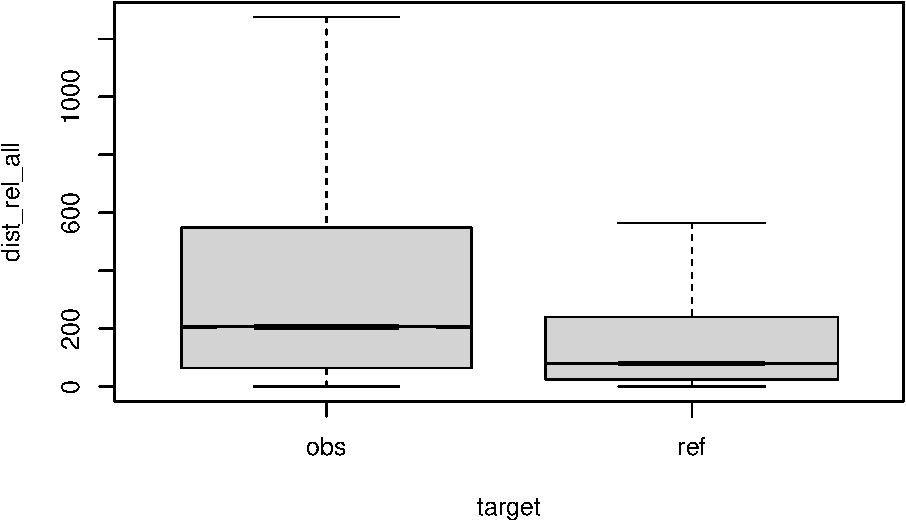
\includegraphics{spund-pub_files/figure-latex/boxplot1-1} \caption{compare distances by corpus, normalised to obs, distance ceiling =  outliers removed}\label{fig:boxplot1}
\end{figure}

\begin{figure}[H]
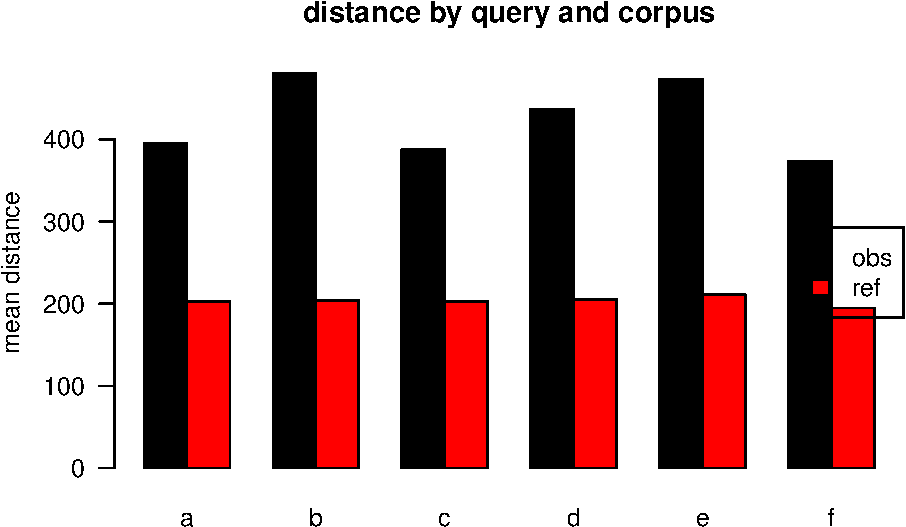
\includegraphics{spund-pub_files/figure-latex/barplot-median-1} \caption{mean distances over query/corpus, normalised to obs, distance ceiling =  outliers removed}\label{fig:barplot-median}
\end{figure}

\begin{longtable}[]{@{}llrrr@{}}
\caption{\label{tab:dfe-table}mean/median table for M13}\tabularnewline
\toprule\noalign{}
target & q & n & mean & median \\
\midrule\noalign{}
\endfirsthead
\toprule\noalign{}
target & q & n & mean & median \\
\midrule\noalign{}
\endhead
\bottomrule\noalign{}
\endlastfoot
obs & a & 42836 & 234 & 117 \\
ref & a & 58615 & 121 & 47 \\
obs & b & 2116 & 286 & 165 \\
ref & b & 1130 & 121 & 44 \\
obs & c & 5770 & 231 & 114 \\
ref & c & 1274 & 120 & 48 \\
obs & d & 5654 & 260 & 144 \\
ref & d & 1525 & 122 & 49 \\
obs & e & 3911 & 281 & 147 \\
ref & e & 671 & 125 & 45 \\
obs & f & 2311 & 222 & 133 \\
ref & f & 413 & 116 & 47 \\
\end{longtable}

\begin{figure}[H]
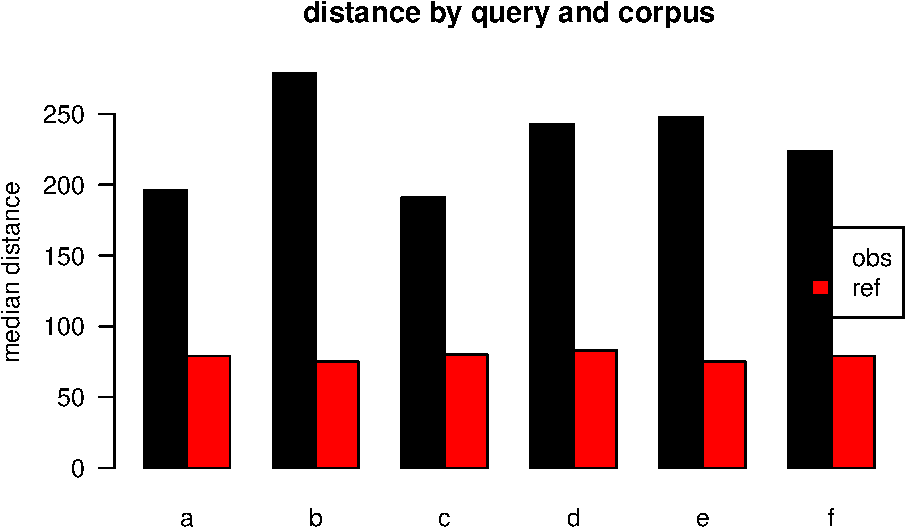
\includegraphics{spund-pub_files/figure-latex/barplot-mean-1} \caption{median distances over query/corpus, normalised to obs, distance ceiling =  outliers removed}\label{fig:barplot-mean}
\end{figure}

\begin{figure}[H]
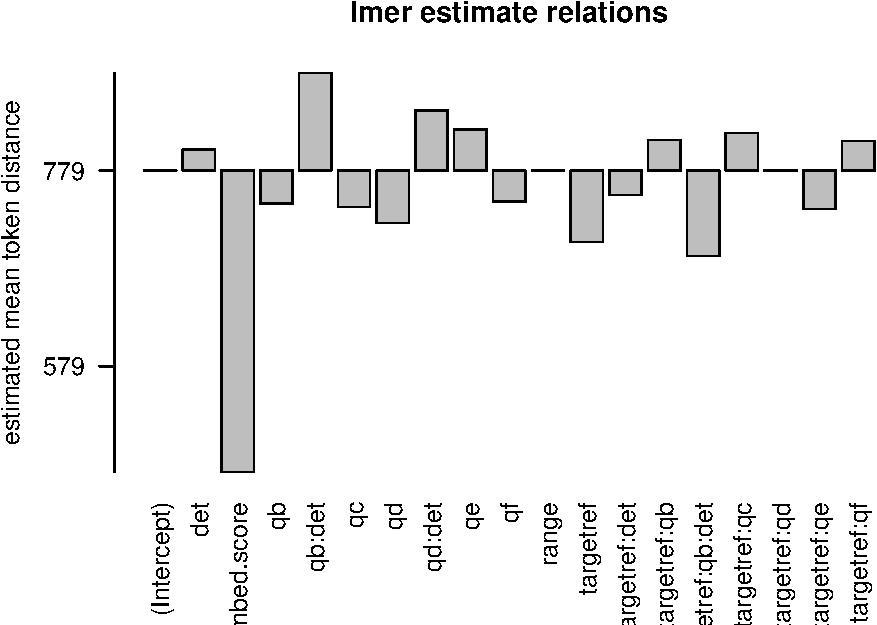
\includegraphics{spund-pub_files/figure-latex/lmeplot-1} \caption{distances relation, normalised to obs, distance ceiling =  outliers removed}\label{fig:lmeplot}
\end{figure}

\begin{figure}[H]
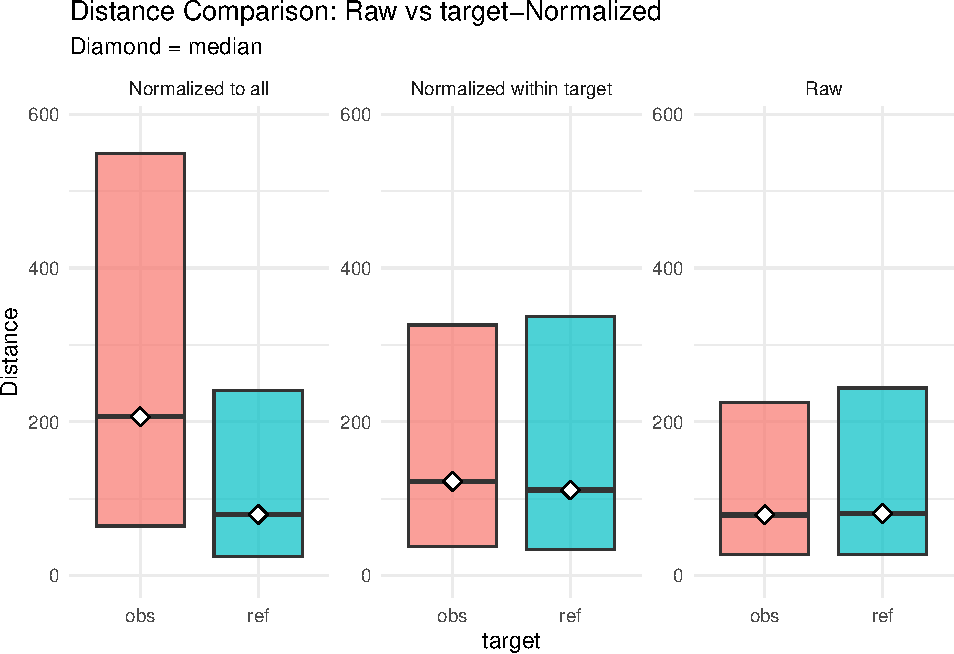
\includegraphics{spund-pub_files/figure-latex/gplot-1} \caption{distances normalised vs. raw}\label{fig:gplot}
\end{figure}

\begin{center}\rule{0.5\linewidth}{0.5pt}\end{center}

\section{REF}\label{ref-1}

literature used and alii\ldots{}

\phantomsection\label{refs}
\begin{CSLReferences}{1}{0}
\bibitem[\citeproctext]{ref-bates_fitting_2015}
Bates, Douglas, Martin Mächler, Ben Bolker, and Steve Walker. 2015. {``Fitting {Linear} {Mixed}-{Effects} {Models} {Using} Lme4.''} \emph{Journal of Statistical Software} 67 (1): 1--48. \url{https://doi.org/10.18637/jss.v067.i01}.

\bibitem[\citeproctext]{ref-de_marneffe_universal_2021}
De Marneffe, Marie-Catherine, Christopher D. Manning, Joakim Nivre, and Daniel Zeman. 2021. {``Universal {Dependencies}.''} \emph{Computational Linguistics}, May, 1--54. \url{https://doi.org/10.1162/coli_a_00402}.

\bibitem[\citeproctext]{ref-huggingface_all-minilm-l6-v2_2025}
HuggingFace. 2025. {``All-{MiniLM}-{L6}-V2 · {Hugging} {Face}.''} \emph{Sentence Transformers}. \url{https://huggingface.co/sentence-transformers/all-MiniLM-L6-v2}.

\bibitem[\citeproctext]{ref-kjell_text-package_2023}
Kjell, Oscar, Salvatore Giorgi, and H. Andrew Schwartz. 2023. {``The Text-Package: {An} {R}-Package for {Analyzing} and {Visualizing} {Human} {Language} {Using} {Natural} {Language} {Processing} and {Deep} {Learning}.''} \emph{Psychological Methods}. \url{https://doi.org/10.1037/met0000542}.

\bibitem[\citeproctext]{ref-kuperberg_language_2010}
Kuperberg, Gina R. 2010. {``Language in Schizophrenia {Part} 2: {What} Can Psycholinguistics Bring to the Study of Schizophrenia\ldots and Vice Versa?''} \emph{Language and Linguistics Compass} 4 (8): 590--604. \url{https://doi.org/10.1111/j.1749-818X.2010.00217.x}.

\bibitem[\citeproctext]{ref-lee_higher-order_2018}
Lee, Kenton, Luheng He, and Luke Zettlemoyer. 2018. {``Higher-Order {Coreference} {Resolution} with {Coarse}-to-Fine {Inference}.''} arXiv. \url{https://doi.org/10.48550/arXiv.1804.05392}.

\bibitem[\citeproctext]{ref-mishara_klaus_2010}
Mishara, Aaron L. 2010. {``Klaus {Conrad} (1905--1961): {Delusional} {Mood}, {Psychosis}, and {Beginning} {Schizophrenia}.''} \emph{Schizophrenia Bulletin} 36 (1): 9--13. \url{https://doi.org/10.1093/schbul/sbp144}.

\bibitem[\citeproctext]{ref-noauthor_nomic-ainomic-embed-text-v15_2024}
{``Nomic-Ai/Nomic-Embed-Text-V1.5 · {Hugging} {Face}.''} 2024. \url{https://huggingface.co/nomic-ai/nomic-embed-text-v1.5}.

\bibitem[\citeproctext]{ref-noauthor_nomic-embed-text_nodate}
{``Nomic-Embed-Text.''} n.d. Accessed October 6, 2025. \url{https://ollama.com/nomic-embed-text}.

\bibitem[\citeproctext]{ref-nussbaum_nomic_2024}
Nussbaum, Zach, John X. Morris, Brandon Duderstadt, and Andriy Mulyar. 2024. {``Nomic {Embed}: {Training} a {Reproducible} {Long} {Context} {Text} {Embedder}.''} \url{https://huggingface.co/nomic-ai/nomic-embed-text-v1.5}.

\bibitem[\citeproctext]{ref-ottiram_ottirammmax2_2025}
ottiram. 2025. {``Ottiram/{MMAX2}.''} \url{https://github.com/ottiram/MMAX2}.

\bibitem[\citeproctext]{ref-poesio_massimo_arrau_2013}
Poesio, Massimo, Artstein, Ron, Uryupina, Olga, Rodriguez, Kepa, Delogu, Francesca, Bristot, Antonella, and Hitzeman, Janet. 2013. {``The {ARRAU} {Corpus} of {Anaphoric} {Information}.''} Linguistic Data Consortium. \url{https://doi.org/10.35111/Y3MR-HE10}.

\bibitem[\citeproctext]{ref-prince_toward_1981}
Prince, Ellen F. 1981. {``Toward a Taxonomy of Given-New Information.''} In \emph{Syntax and Semantics: {Vol}. 14. {Radical} {Pragmatics}}, edited by P. Cole, 223--55. New York: Academic Press.

\bibitem[\citeproctext]{ref-rivera_redditextractor_2023}
Rivera, Ivan. 2023. {``{RedditExtractoR}: {Reddit} {Data} {Extraction} {Toolkit}.''} \url{https://CRAN.R-project.org/package=RedditExtractoR}.

\bibitem[\citeproctext]{ref-schwarz_poster_2025}
Schwarz, St. 2025. {``Poster Appendix: This Papers Scripts for Corpus Build and Statistics on Github.''} \url{https://github.com/esteeschwarz/SPUND-LX/tree/main/psych/HA}.

\bibitem[\citeproctext]{ref-wijffels_udpipe_2023}
Wijffels, Jan. 2023. \emph{Udpipe: {Tokenization}, {Parts} of {Speech} {Tagging}, {Lemmatization} and {Dependency} {Parsing} with the '{UDPipe}' '{NLP}' {Toolkit}}. \url{https://CRAN.R-project.org/package=udpipe}.

\bibitem[\citeproctext]{ref-zimmerer_deictic_2017}
Zimmerer, Vitor C., Stuart Watson, Douglas Turkington, I. Nicol Ferrier, and Wolfram Hinzen. 2017. {``Deictic and {Propositional} {Meaning}---{New} {Perspectives} on {Language} in {Schizophrenia}.''} \emph{Frontiers in Psychiatry} 8 (February). \url{https://doi.org/10.3389/fpsyt.2017.00017}.

\end{CSLReferences}

\end{document}
